\section{Experimental methods and data post-processing}

\subsection{Tissue sources and experimental methods} \label{c3:sec:21}

    Details of the tissue source, preparation and mechanical evaluation have been previously presented \cite{sun_biaxial_2003}. Briefly, large sections of native bovine pericardium were stored in phosphate-buffered saline (pH 7.4) at $4^\circ C$, then optically cleared using a hyperosmotic solution and the collagen fibre architecture (CFA) quantified. From the resulting CFA information, $25\times25$ mm test specimens exhibiting a high degree of structural uniformity suitable for biaxial testing were selected. The collagen fibre preferred and cross-preferred directions were aligned to the $X_1$-$X_2$ axes (figure \ref{c3:fig:3}). A total of five specimens were prepared in the native state.
    
%%%%%%%%%%%%%%%%%%%%	begin FIGURE 	%%%%%%%%%%%%%%%%%%%%
\begin{figure}
\centering
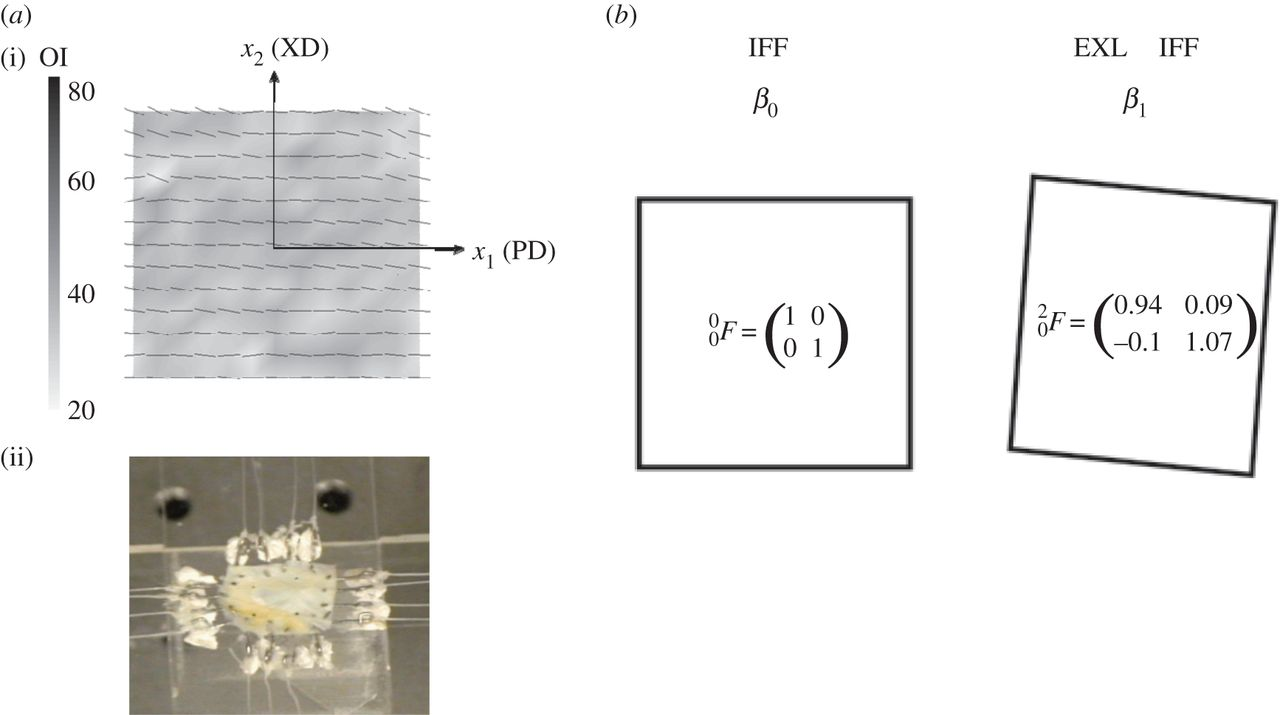
\includegraphics[width=\textwidth]{Images/chapter3/F3large.jpg}
\caption{a)(i) Pericardial test specimen showing a high degree of fibre orientation and uniformity in preferred fibre directions, with the PD = $X_1$ and XD = $X_2$ axes defined, and (ii) a typical biaxial test specimen mounted on the device. (b) A schematic of the biaxial test specimen geometry changes with cross-linking and the corresponding mean deformation gradient tensor components in native state $\beta_0$ and EXL state state $\beta_1$. Here, cross-linking induced a 6\% contraction in the PD and and 7\% direction in the XD, with some small shearing.}
\label{c3:fig:3}
\end{figure}
%%%%%%%%%%%%%%%%%%%%	 end FIGURE 	%%%%%%%%%%%%%%%%%%%%

    Biaxial mechanical testing methods have been previously described in detail \cite{sacks_orthotropic_1998,sacks_method_1999}. Briefly, testing was performed with the specimen immersed in phosphate-buffered normal saline (pH 7.4) at room temperature. First the Piola Kirchhoff stress $\mathbf{P}$ controlled test protocol was used, wherein the ratio of the normal stress components $P_{11}$:$P_{22}$ was kept constant, with $P_{12} = P_{21} = 0$ and a maximum stress level of 1 MPa was used. Tissue deformations were quantified from the motion of four markers placed in the central third of the specimen, from which the deformation gradient tensor $\mathbf{F}$ was determined. For the first testing phase, an equi-biaxial stress protocol (i.e. $P_{11}$:$P_{22}$ = 1 : 1) was used for both preconditioning and data acquisition. A total of 15 contiguous cycles were run with an approximate strain rate of 0.01 $s^{-1}$. Next, seven successive protocols were performed using ratios $P_{11}$:$P_{22}$ = 1 : 0.1, 1 : 0.5, 1 : 0.75, 1 : 1, 0.75 : 1, 0.5 : 1 and 0.1 : 1. This range was chosen for extensive coverage of in-plane strain state. After testing, each native specimen was allowed to mechanically re-equilibrate by storing them in a stress-free state at $4^\circ C$ for 24 h. Next, each specimen was chemically treated with 0.625\% GLUT for a minimum of 72 h, with the tissue marker dimensions monitored throughout the cross-linking procedure, and then stored in phosphate-buffered normal saline at $4^\circ C$. As a final step, the above biaxial testing sequence was repeated. Data post-processing included computation of the second Piola-Kirchhof tensor $\mathbf{S}$ and deformation gradient tensor $\mathbf{F}$ using established methods \cite{zhang_generalized_2015}. This test design allowed a comprehensive planar mechanical behaviour dataset to be collected on matched native and EXL specimens, compensating for inter-specimen variations.
    
    
    
    
\subsection{Kinematic considerations and mechanical data post-processing}

    As observed in our other studies \cite{sacks_biaxial_2000,zhang_generalized_2015}, the chemical fixation process will affect the specimen dimensions, and any analysis must carefully account for these effects on the collagen fibre kinematics. We thus defined the following configurations: $\beta_0$-native, $\beta_1$-EXL (figure \ref{c3:fig:3}b), used as the referential configurations for the native and EXL states, respectively. We represented all deformations using the notation for the deformation gradient tensor $\prescript{j}{i}{\mathbf{F}}$ where $i$ and $j$ represent the initial and final configurations, respectively (Nomenclature). Values for the components of $\prescript{j}{i}{\mathbf{F}}$ were determined using the same method from section \ref{c3:sec:21} for the displacements of the four markers pre- and post-cross-linking for each specimen. Next, as first described by Lanir \cite{lanir_constitutive_1983}, we defined a fibre ensemble as a group of fibres with a common orientation. It has been shown that the ensemble stress–strain relation can be obtained from the interpolated equi-biaxial strain path, where $\mathbf{F} = \operatorname{diag}[\lambda, \lambda, 1/\lambda^2]$ using $S_{ens} = S_{11} + S_{22}$ \cite{sacks_incorporation_2003}. To derive the equi-biaxial strain path $\lambda_1 = \lambda_2$ from the stress-controlled experimental data, all mechanical data were combined and interpolated using cubic Hermite patches \cite{fata_insights_2014}. A strain path with $\lambda_1 = \lambda_2$ was interpolated within the range of the data as defined by the convex hull of ($\lambda_1$, $\lambda_2$), and was implemented separately for each stress component (figure \ref{c3:fig:4}). To reliably overcome regions of sparse data we enforced the surface to be strictly convex everywhere. Finally, since the $S_{12}$ component was negligible in all specimens, it was ignored in the subsequent analyses.
    
    
%%%%%%%%%%%%%%%%%%%%	begin FIGURE 	%%%%%%%%%%%%%%%%%%%%
\begin{figure}
\centering
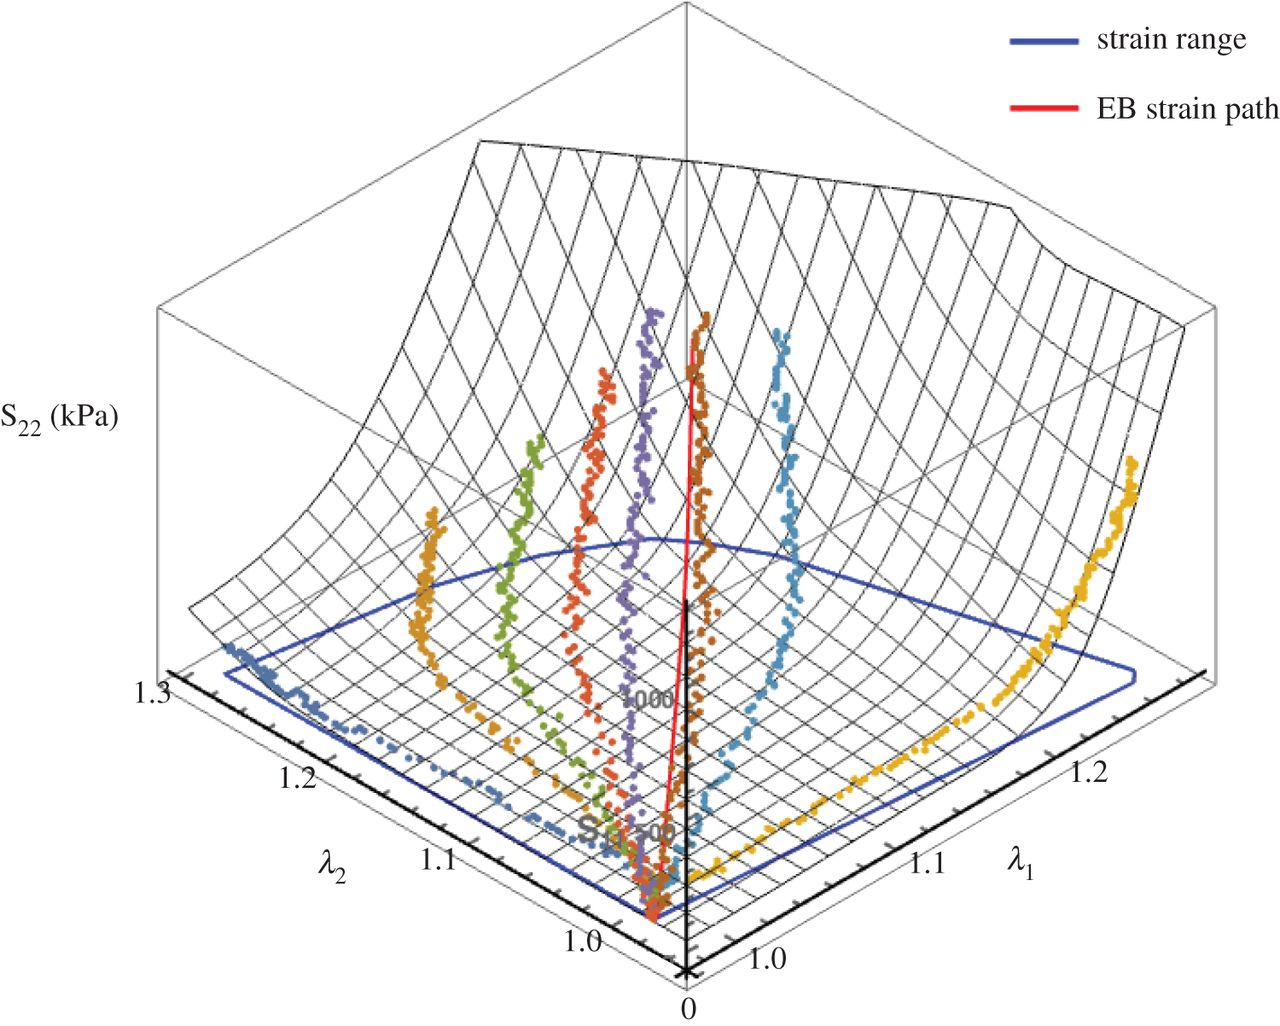
\includegraphics[width=\textwidth]{Images/chapter3/F4large.jpg}
\caption{An example of the bicubic Hermite surface interpolation of the $S_{22}$ biaxial test responses to allow interpolation of an equi-biaxial strain path, shown here in red. The blue path defines the span of the strain.}
\label{c3:fig:4}
\end{figure}
%%%%%%%%%%%%%%%%%%%%	 end FIGURE 	%%%%%%%%%%%%%%%%%%%%
    


\subsection{Establishing and modelling the mechanical behaviour of the native collagen fibre ensemble}
    
    Based on our previous tissue model findings \cite{sacks_incorporation_2003,fata_insights_2014,fan_simulation_2014,lee_presence_2015}, the dominant cause of the nonlinearity of the tissue-level mechanical behaviour of collagenous tissues is the gradual recruitment of collagen fibres \cite{lanir_constitutive_1983}. The collagen fibres themselves behave linearly under typical fibre strains experienced under physiological stresses in tissues (2–5\%). 
    Once all fibres are fully straightened, the summed response should appear linear in the ensemble response. When applied to the equi-biaxial strain derived fibre-ensemble data, the upper bound can be directly determined as the transition point between the nonlinear and linear regions, with the slope of the linear region establishing the maximum tangent modulus (MTM) of the collagen fibre ensemble (e.g. \cite{fata_insights_2014}). The matrix response can also be determined from the pre-recruitment region where no collagen fibre have contributed. To determine the recruitment upper bound in the native tissue, we started at the largest measured strain and decreased the strain level until the region above was no longer linear. Linearity was defined from the mean squared error (MSE) of the linear regression to be less than 0.005\% of the total MSE of all data, where $\mathrm{MSE} = \sum_i^n (\mathrm{S}^i_{ens} - \bar{\mathrm{S}}_{ens})/n$. Similarly, we determined the lower bound by starting at zero strain and increasing the strain until a deviation from linearity was determined.
    
    
    Next, we note that in some previous structural models a fibre stress–strain relation linear in the second Piola-Kirchhoff stress and Green Lagrange strain has been used \cite{sacks_incorporation_2003,fan_simulation_2014,lanir_structural_1979}. However, SAXS studies have demonstrated a linear force\Hyphdash displacement relation for collagen fibrils in the tendon \cite{sasaki_elongation_1996,sasaki_stress_1996} and MV tissue \cite{liao_relation_2007}. This is further corroborated by the atomistic modelling results by Buehler \cite{buehler_atomistic_2006}, where the force\Hyphdash displacement relation is essentially linear at strains lower than 0.35. We have recently determined that for the mitral valve leaflet the tissue level-derived collagen fibre mechanical behaviour is actually quite linear, with an effective modulus of approximately 160 MPa. Based on these considerations, we assumed for the native collagen fibres that
        \begin{enumerate}
            \item they exhibit a linear $P-\lambda$ response
            \item slack stretch of the collagen fibres does not vary with orientation.
        \end{enumerate}
    From these two basic considerations, we used the following effective native collagen fibre model \cite{fata_insights_2014,fan_simulation_2014}. We start by defining the native collagen fibre strain energy as
        %-------------------	begin EQUATION 	-------------------%
        \begin{equation}\label{c3:eqn:21}
        \begin{aligned}
        \Psi_f(\lambda_t) = 
            \begin{cases} 
                \frac{\eta_c}{2} \left(\lambda_t -1\right)^2 & \text{for } \lambda_t >1\\
                0 & \text{for } \lambda_t < 1  
            \end{cases}
        \end{aligned}
        \end{equation}
        %-------------------	 end EQUATION 	-------------------%
    where $\lambda_t = \lambda_f/\lambda_s$ is the true stretch of the fibre. This leads to the following $P-\lambda$ form using $P_f = \partial \Psi_f(\lambda_t)/\partial \lambda_f = \partial \Psi_f(\lambda_t)/\partial \lambda_t \cdot \partial \lambda_t/\partial \lambda_f$
        %-------------------	begin EQUATION 	-------------------%
        \begin{equation}\label{c3:eqn:22}
        \begin{aligned}
        P_f = 
            \begin{cases} 
                \frac{\eta_c}{\lambda_s} \left(\lambda_t -1\right) & \text{for } \lambda_t >1\\
                0 & \text{for } \lambda_t < 1  
            \end{cases}
        \end{aligned}
        \end{equation}
        %-------------------	 end EQUATION 	-------------------%
    where $P_f$ is the first Piola-Kirchhoff stress of the fibre, $\eta_c$ is the modulus of the fibre, $\lambda_f$ is the fibre stretch and $\lambda_s$ is the fibre slack stretch. Next, we use this fibre model in the expression for the native collagen fibre ensemble using
        %-------------------	begin EQUATION 	-------------------%
        \begin{equation}\label{c3:eqn:23}
        \begin{aligned}
        P_c^{ens} =& \phi_c\eta_c\int_1^{\lambda_\theta}\frac{D(x)}{x} \left(\frac{\lambda_\theta}{x} - 1\right) \dif x    \\
        \text{and} \quad \dpd{P_c^{ens}}{\lambda_\theta} =&\mathrm{TM}_c^{ens} = \phi_c\eta_c\int_1^{\lambda_\theta}\frac{D(x)}{x^2}\dif x,
        \end{aligned}
        \end{equation}
        %-------------------	 end EQUATION 	-------------------%
    where $\phi_c$ is the collagen fibre mass fraction, $\lambda_\theta$ is the fibre-ensemble stretch along the direction defined by $\theta$ (computed from the tissue-level deformation using $\lambda_\theta = \mathbf{F}\cdot\mathbf{n}(\theta)$), and $D(\lambda_s)$ is the probability distribution function describing the distribution of collagen fibre slack length within the ensemble. We assumed $D(\lambda_s)$ is Beta distributed, so that
        %-------------------	begin EQUATION 	-------------------%
        \begin{equation}\label{c3:eqn:24}
        \begin{aligned}
        D(\alpha, \beta, \lambda_{lb}, \lambda_{ub}, \lambda_s) =& 
            \begin{cases}
            \frac{y^{\alpha-1}(1-y)^{\beta-1}}{B(\alpha,\beta)(\lambda_{ub}-\lambda_{lb})} & \text{for } y \in [0,1] \\
            0 & \text{otherwise}
            \end{cases} \\
        y=&\frac{\lambda_s-\lambda_{lb}}{\lambda_{ub}- \lambda_{lb}}, \quad \bar{\mu} =\frac{\mu - \lambda_{lb}}{\lambda_{ub}-\lambda_{lb}}   \\
        and \quad \bar{\sigma} =& \frac{\sigma}{\lambda_{ub} - \lambda_{lb}}, \quad \alpha = \frac{\bar{\mu}^2 - \bar{\mu}^3 - \bar{\sigma}^2\bar{\mu}}{\bar{\sigma}^2},   \\
        \beta =& \alpha \frac{1-\bar{\mu}}{\bar{\mu}}
        \end{aligned}
        \end{equation}
        %-------------------	 end EQUATION 	-------------------%
    where $\lambda_{lb}$ and $\lambda_{ub}$ are the lower and upper bound stretch of the collagen fibre recruitment, respectively. Note that in preliminary examinations of the data we found that all specimens exhibited distinct pre- and post-transition locations (figure \ref{c3:fig:5}), allowing $\lambda_{lb}$ and $\lambda_{ub}$ to be determined directly from the collagen fibre ensemble data. Thus, the complete initial ensemble model (equation \ref{c3:eqn:23}) has three parameters $\{\eta_c, \alpha, \beta\}$ to fit to the data using standard techniques \cite{fata_insights_2014}.
    
    
    
    
    
%%%%%%%%%%%%%%%%%%%%	begin FIGURE 	%%%%%%%%%%%%%%%%%%%%
\begin{figure}
\centering
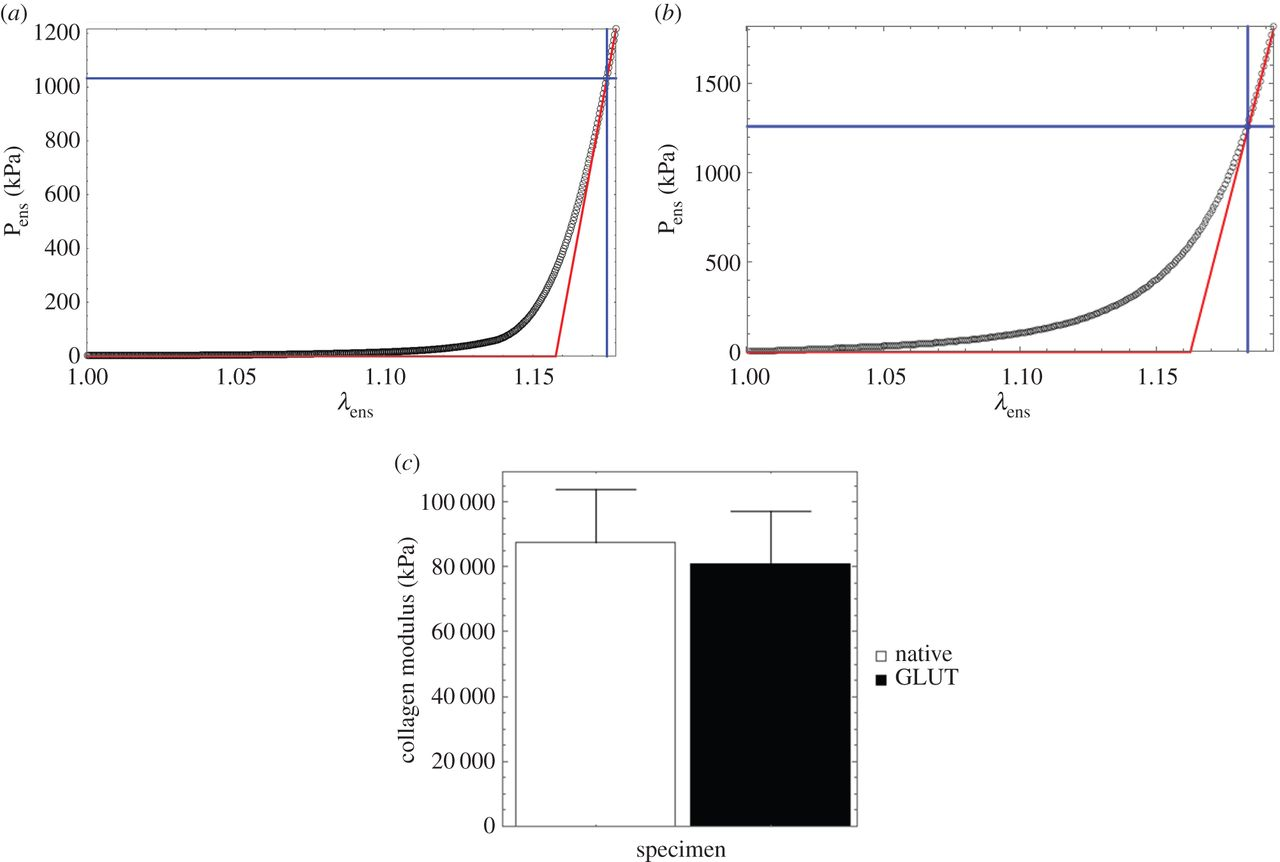
\includegraphics[width=\textwidth]{Images/chapter3/F5large.jpg}
\caption{A representative fibre-ensemble stress–strain (in $P_\mathrm{ens}-\lambda_\mathrm{ens}$) response for (a) native and (b) cross-linked bovine pericardium illustrating a well-defined post-transition fibre recruitment point wherein the response becomes linear. While the native pericardium demonstrated a very low initial modulus (approx. 75 kPa; table \ref{c3:tab:2}), the EXLs demonstrate a significantly stiffer modulus.}
\label{c3:fig:5}
\end{figure}
%%%%%%%%%%%%%%%%%%%%	 end FIGURE 	%%%%%%%%%%%%%%%%%%%%